%!TEX ROOT = thesis.tex
\chapter{Framework Overview}
\label{chapter:framework}
\section{Introduction}
In order to tackle the issues identified through the research questions and literature review, the theoretical framework is laid as to provide a conceptual schema to break the rather huge and intricate challenge into multiple bite sized puzzles. First, the overview of the proposed framework used in this work is described in Section \ref{section:framework}. Next, the description of the dataset used is given in Section \ref{section:dataset_used} and finally, this chapter concludes with the experimental methodology applied to obtain the results (see Section \ref{sec:expmethodology}).


\section{Framework Overview}
\label{section:framework}
In this section, a high level overview of the fundamental processes along with two suggested core components for vehicle semantic extraction and retrieval is provided.
The groundwork described in this work abides to the typical top-down approach used in Intelligent Transportation System (ITS) where the video data is subjected to background subtraction, followed by blob filtering, vehicle detection as well as vehicle tracking is as described in \cite{lim2017}.
The semantic information from the vehicle blobs are then extracted and stored in the database.

Now, with the vehicle specific semantics stored in the database, retrieval engines were designed to enabled users to easily retrieve the stored information. Both retrieval engines features a graphical user interface which allows users to enter the queries by drawing the desired trajectory on the search interface as well as providing other crucial information which would assist in identifying the targeted video shot.

However, as mentioned in Section \ref{subsec:scope}, the bounding box of the vehicles are assumed to be obtained prior to the semantic extraction task. Hence, the semantic extraction and video retrieval processes are the central emphasis of this work.

\begin{figure}[hbt!]\centering
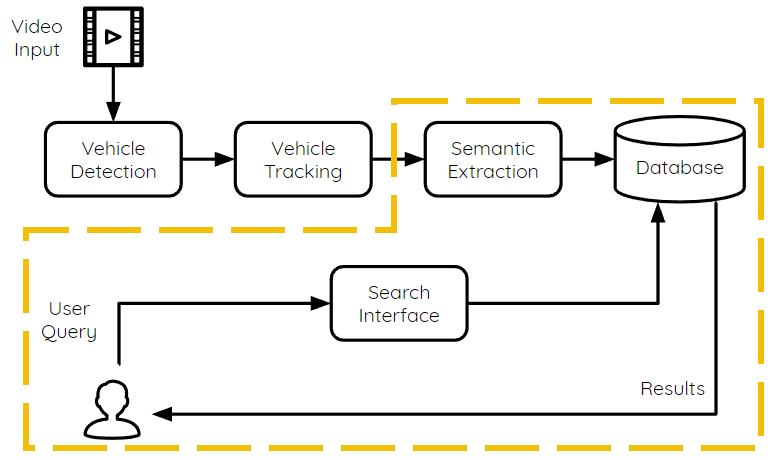
\includegraphics[width=.9\textwidth]{image/new/framework_new.PNG}
\caption{Framework Diagram, Contribution in Highlighted Border}
\label{fig:framework}
\end{figure}


In this work, a frameworks was suggested and used for the vehicle semantic extraction and retrieval process.
As mentioned in the first chapter, the proposed methods were developed in two cascading phase with the same objective.
The formulation of idea, steps and process involved in each phase is described in this chapter.
As a whole, the end-to-end framework can be visualised using Figure \ref{fig:framework} where the main contribution of this work is highlighted in yellow border.

\subsection{Phase 1: LSH-Inspired Semantic Extraction and Retrieval Technique}
\label{subsec:lsh-intro}
The first of the two techniques suggested in this work is the \textit{LSH-Inspired Semantic Extraction and Retrieval Technique}. Locality-Sensitive Hashing (LSH) is a technique used for dimensionality reduction.
Unlike conventional hashing techniques that aims to avoid hash collision, LSH tries to maximize hash collisions.
When performed on a set of documents, documents with similar properties are mapped and clustered to similar locality or neighbourhood. This technique excels especially when working with high dimensional data such as video data.

However, the exact implementation of LSH was not done in this work. Instead, inspirations to cluster similar documents were drawn and implemented in this phase. The extracted semantics from each vehicle blobs were clustered into semantic groups of 11 colours and 9 motion clusters. This concept was adopted in the proposed method with the following considerations in mind:

\begin{enumerate}
    \item Ease of Interpretation \& Access: As the extracted semantics are stored in clusters of similar properties, these semantics can be easily interpreted and retrieved.
    \item Reduction of Input/Output (I/O) Bottleneck: As the proposed method stores the extracted semantics in a database, I/O bottlenecks are bound to occur when reading and retrieving large quantity of data. Given that semantics of similar properties were clustered together, the retrieval technique only has to search through the the matching tables instead of the entire database for matching records.
\end{enumerate}


\subsection{Phase 2: CD-Inspired Semantic Extraction and Retrieval Technique}
The second technique suggested in this work is the \textit{Chamfer Distance-Inspired Semantic Extraction and Retrieval Technique}.
Chamfer Distance (CD) is one of the many distance measure (see Section \ref{section:distancemeasures}) introduced by mathematicians and researchers. Chamfer Distance, as introduced by \cite{barrow1977parametric}, was originally designed to match images by comparing the shapes of two collections of shape fragments.
However, in this work, the use of chamfer distance was modified to suit the research problem of comparing vehicle trajectories' shapes. While the implementation of chamfer distance measure in this framework has its advantages, it also comes with some drawbacks. The considerations taken when designing this technique is as such:

\begin{enumerate}
    \item The use of Chamfer Distance to compare trajectories allows the retrieval technique to search from a wider range. While this comes with extra computational cost which are undesirable, the increased robustness outweighs the drawback. Along with that, the use of time and date filtering could potentially reduce the number of records, hence, further reducing the computational cost.
    \item The ranking of results is a desirable feature in a retrieval engine. As Chamfer Distance produces a distance score for every pair of trajectories compared, this score can be used to sort the results in an intuitive manner where results of higher resemblance would appear higher in the ranking.
\end{enumerate}


\section{Dataset}
\label{section:dataset_used}

In view of testing the proposed framework, a new video dataset was gathered as there are limited public long-term car park dataset. A stationary cloud-enabled web camera was set up in a room on the fourth floor of a building facing a piece of private car park area. Figure \ref{fig:camerasetup} depicts the camera setup overcasting the car park area.

%The aforementioned setup was done to mimic a typical camera setup which tower over a piece of outdoor car park lot that are found in the wild.


\begin{figure}[hbt!]\centering
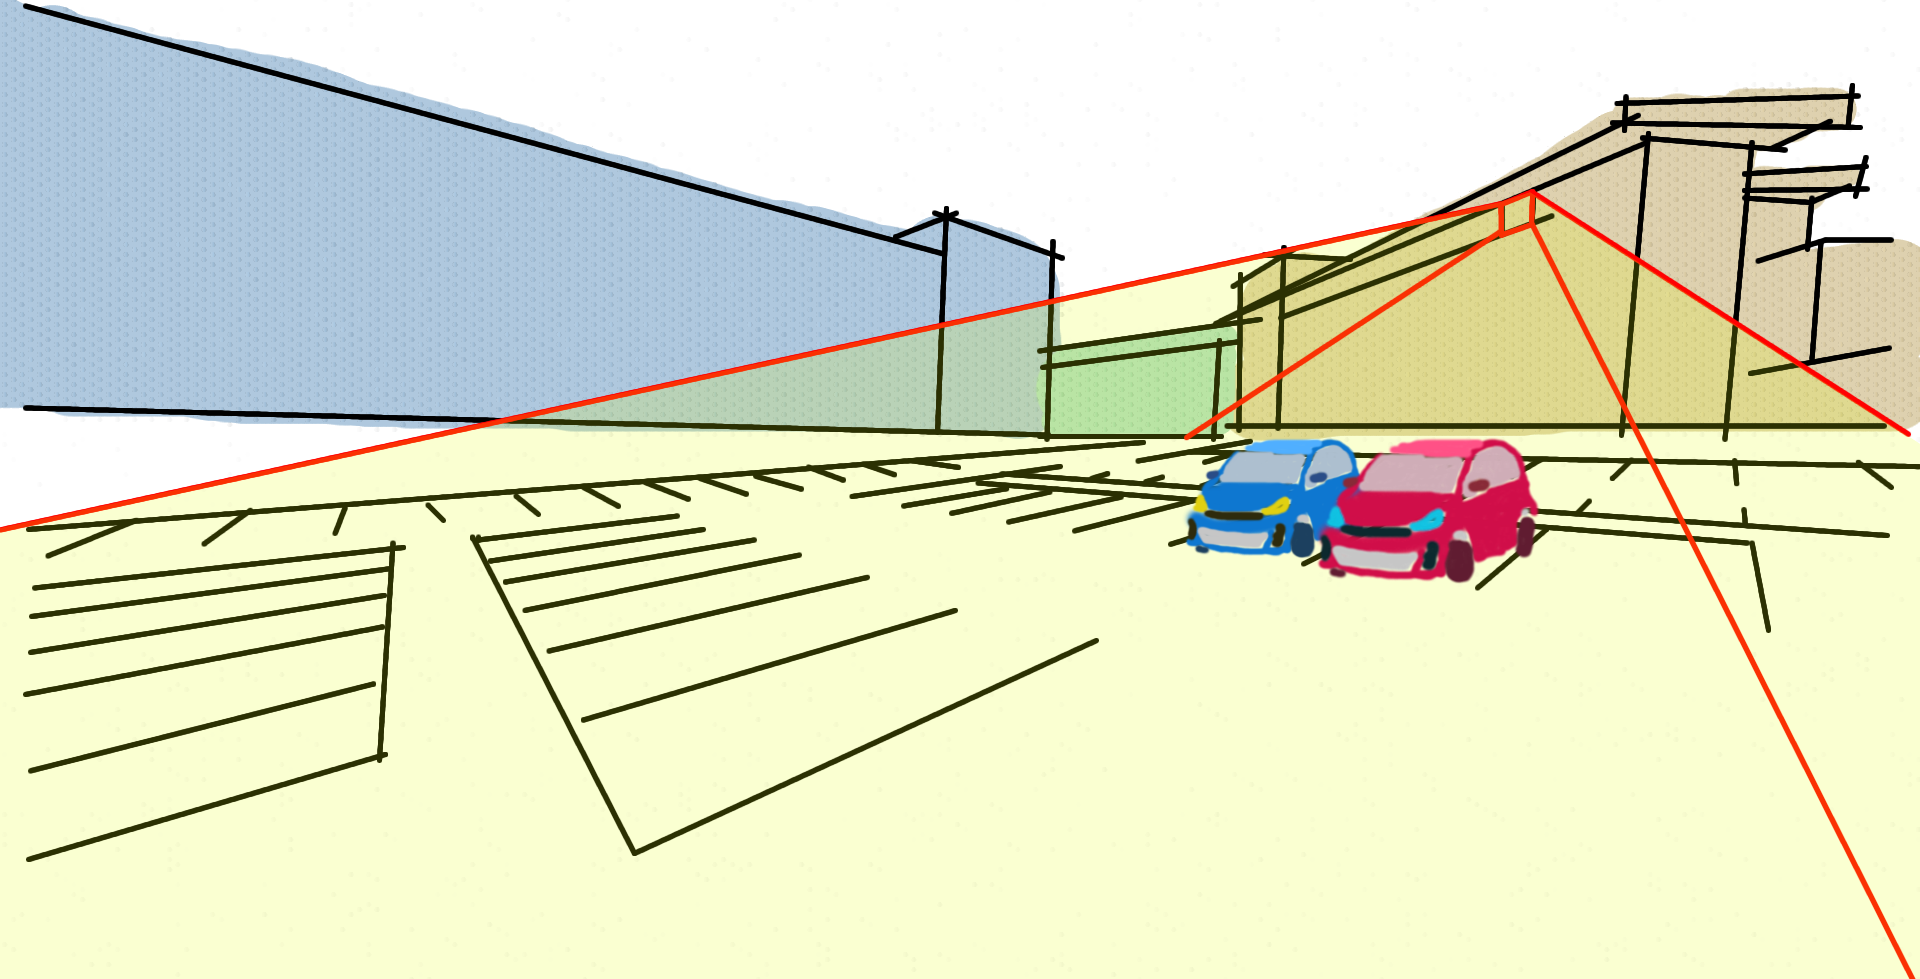
\includegraphics[width=.8\textwidth]{image/new/fcicarpark2.png}
\caption{Camera setup to capture the car park from the fourth floor}
\label{fig:camerasetup}
\end{figure}


\begin{figure}[!hbt]\centering
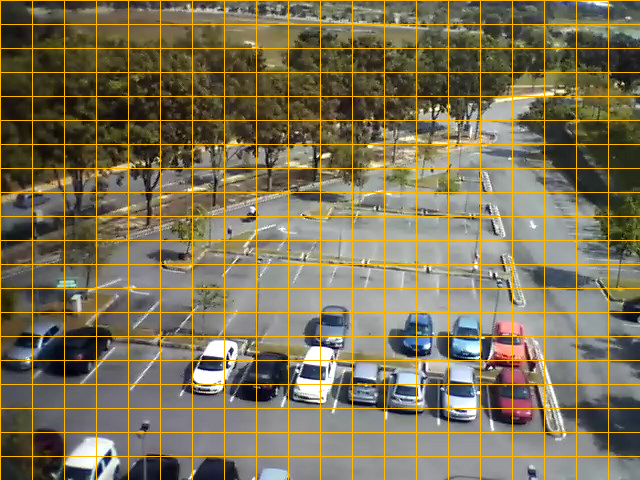
\includegraphics[width=.7\textwidth]{image/general/grids.png}
\caption{View from camera setup; 20$\times$20 Grids}
\label{fig:viewfromcamera}
\end{figure}


Through the camera's web interface, the device was set to record on weekdays from Monday through Friday, starting from 08:30am in the morning up until 18:30pm in the evening, with a total of 10 hours of video recorded each day. As each recorded video clip was set to have a maximum length of 6 minutes, a total of 100 videos were obtained at the end of each day. The recorded video clips were saved unto a microSD memory card.
At the end of each day, the data was copied over to a server via a script. However, due to glitches that occurred during the recording process, some of the video clips were cut off abruptly. Hence, some of the days does not contain the full 10 hours video clips.

\begin{table}[!ht]\centering
\begin{tabular}{ll}
Camera Model: & Dlink DSC-942L        \\
Resolution:   & 640$\times$480 pixels \\
Frame rate:   & 10 $fps$             \\
Format:       & H.264 / MPEG-4 AVC    \\
Naming Convention: & $CCYYMMDD\_HHMMSS.mp4$
\end{tabular}
\vspace{1em}
\caption{Details of the Camera Setup used for Data Collection}
\end{table}

\begin{figure}[!htb]
  \centering

\begin{tabular}{cc}
 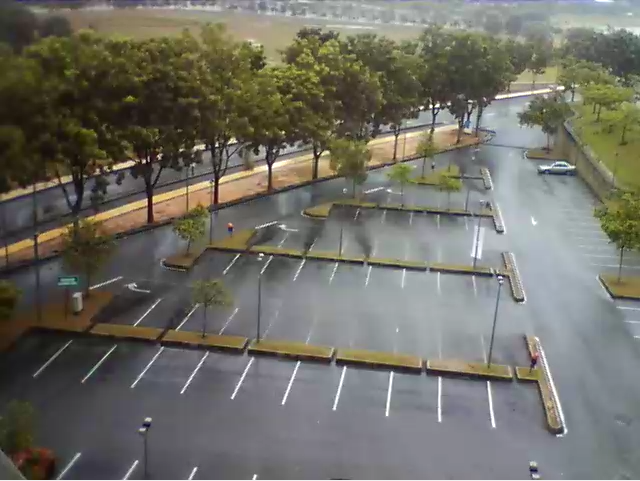
\includegraphics[width=0.4\linewidth]{image/general/rain.PNG} &  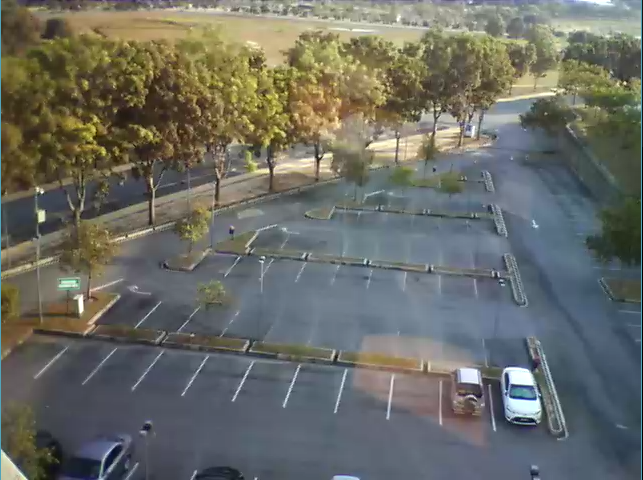
\includegraphics[width=0.4\linewidth]{image/general/reflection.PNG}\\
\begin{tabular}{c}(a) Rainy day with \\ reflective surface\end{tabular} & \begin{tabular}{c}(b) Reflection on the \\car park from the window\end{tabular} \\
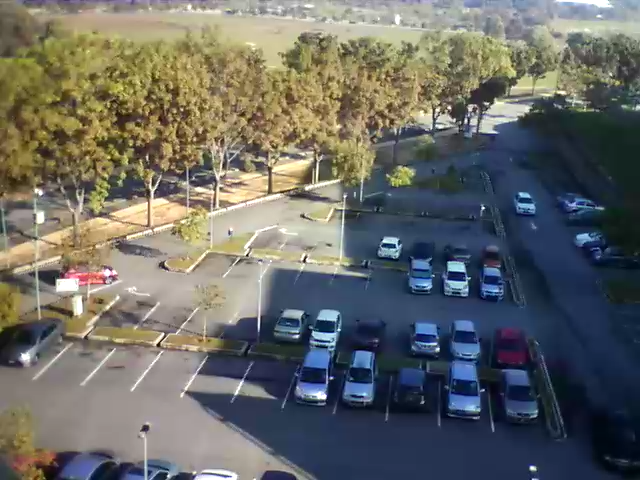
\includegraphics[width=0.4\linewidth]{image/general/shadow.png} &  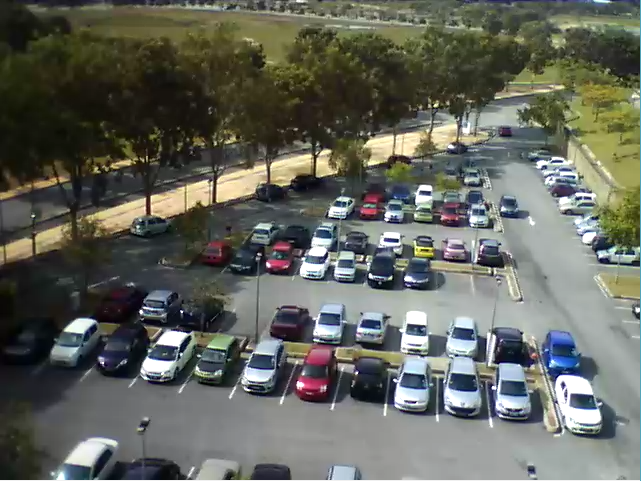
\includegraphics[width=0.4\linewidth]{image/general/shadow2.png}\\
\begin{tabular}{c}(c) Severe shadow over \\ the car park (08:48AM)\end{tabular} & \begin{tabular}{c}(d)  Severe shadow over \\ the car park (04:06PM)\end{tabular}
\end{tabular}


\caption{Noisy Data Within the Collected Dataset} \label{fig:weather}
\end{figure}


This setup was left to record data over the course of several months with various weather and lighting conditions. This also includes diverse set of car park scenes such as peak hours with plenty of vehicles along with the off days. Along with that, this setup covers a total of over 45 parking lots excluding parking lots that are too small or occluded. Figure \ref{fig:weather} illustrates the various weather conditions and noise which were recorded sporadically throughout the dataset.


\section{Experimental Methodology}
\label{sec:expmethodology}

In the subsequent chapters, the detailed descriptions of the proposed vehicle semantic extraction algorithm as well as the retrieval techniques will be provided. This section briefly describes the methodology and the experimental setup to provide an overview on how the experiments were performed in this work.

As the performance of the proposed methods are essential towards end users, each of the proposed algorithm in the framework was evaluated with the help of volunteers.
The bounding box obtained using the Vehicle Detection and Vehicle Tracking framework proposed by \cite{lim2017} included errors. While these errors were propagated to the Vehicle Semantics Extraction and Retrieval modules, they were not overlooked nor discarded during the evaluation process. This was done intentionally to provide an end-to-end assessment of the framework.

The proposed methods were implemented and evaluated on an Intel i7 machine with 16GB RAM, equipped with a GeForce GTX 1060 GPU. As the main focus of the proposed method revolves around the semantic extraction and retrieval of \textbf{vehicle colour} along with the \textbf{vehicle trajectory}, both of these components were assessed and evaluated individually.
This was done to better understand the performance, effectiveness as well as the weakness of the proposed methods.

As a result, two different phase was introduced to enhance the performance based on the intels obtained and gaps which were identified. This also allowed us to gain deeper understanding of the proposed method along with the opportunities for future improvements.
Likewise, the experimental methodology can be divided into two phases.
%Two retrieval techniques were designed and implemented in this work, the objective of the first retrieval engine was to build a prototype for the evaluation of the its current performance and to identify gaps to be improved. This process allowed the author to return to the drawing board and reevaluate the algorithms, metrics and evaluation process performed.


\subsection{Phase 1: LSH-Inspired Semantic Extraction and Retrieval Technique (Prototyping)}
While the collected dataset comprised of several months of data, only two days of data (20 hours) were used for the evaluation of \versionOneRet. Several annotators were deployed to manually label and fully annotate these data. Upon completing the annotation process, the annotators would cross-check to verify the sanctity of the annotation.
Along with that, the cross-checking allows the annotators to arrive at consensus on annotations that did not tally. The annotators were asked to take note of following events:
1) Number of vehicle of each colour category (11 categories, see \ref{table:colorshex}), and 2) Number of vehicles performing motion $TQ1$ \& $TQ2$ (See Figure \ref{fig:versionOneInterface}).
Having fully annotated data allowed us to evaluate the performance of the proposed method using the Accuracy, Recall and $F_1$ Score metrics.

\subsection{Phase 2: CD-Inspired Semantic Extraction and Retrieval Technique (Full Experiment)}

During the \textbf{Phase 1} experiment, it was noted that the entire annotation process took a significant amount of work despite only using two days of data. As one month of data was set aside for the evaluation of the \versionTwoRet, an alternative experimental methodology was applied.
Typical with any large-scale retrieval engine of all intents and purposes, it is not feasible to annotate huge amount of ground truth manually as it takes an enormous and time consuming effort.
Hence in \textbf{Phase 2}, semantics from one month of data was extracted, retrieved and evaluated without the manual annotations of any events.

As the final output of this work is a end-user facing retrieval system, the evaluation process took on an empirical user study approach. This unbiased approach provided the volunteers with full control and freedom to perform any kinds of query over the search interface.
Using this setup, a group of six volunteers were performed a total of 11 queries on the retrieval engine for both the vehicle colour and trajectory semantics.
%of the vehicles and provide relevance score for each retrieved results.
Based on each query, the volunteers were tasked to provide relevance score($REL$) and evaluation for each of the randomly ordered retrieved results.
As the data in this phase was not fully annotated, it is impossible to compute the Recall and $F_1$ score. Instead, the Precision@K along with the normalised Discounted Cumulative Gain (nDCG) metrics were used.

